\documentclass[a4paper,oneside,english,reqno]{amsbook}
\usepackage[T1]{fontenc}
\usepackage[latin9]{inputenc}
\synctex=-1
% \usepackage{color}
\usepackage{babel}
\usepackage{textcomp}
\usepackage{mathrsfs}
\usepackage{url}
\usepackage{amstext}
\usepackage{amsthm}
\usepackage{amssymb}
\usepackage{stmaryrd}
\usepackage{tikz}
\usepackage{float}
\usepackage{pgfplots}
\usepackage{graphicx}
\makeindex
\usepackage[all]{xy}

\usepackage{agt}
\hypersetup{pdftitle={Algebraic General Topology and Discontinuous Analysis. Volume 1},
 pdfauthor={Victor Porton},
 pdfsubject={general topology},
 pdfkeywords={discontinuous analysis,discontinuous calculus,algebraic general topology,quasi-uniform spaces,generalizations of proximity spaces,generalizations of nearness spaces,generalizations of uniform spaces}}
% \usepackage{forwardref}
\numberwithin{section}{chapter}

% with \usepackage it fails with new TeX versions,
% without it fails with old ones. So I do neither.
% \usepackage{chngcntr}
% \counterwithout{figure}{chapter}

% Eliminate hyperref warnings: http://tex.findincity.net/view/635399273629833626247444/hyperref-token-not-allowed-warning-possible-bug
\pdfstringdefDisableCommands{%
  \let\enspace\empty  % this causes the warning for \kern
  \let\noindent\empty % this causes the warning for \indent
}

\AtEndDocument{\refstepcounter{thm}\label{finalthm}} % used in addons.tex

% \everymath{\color{blue}}

\begin{document}

\noindent
\href{https://teachsector.com/limit/}{\includegraphics[scale=0.3]{img/Teach-Sector.jpeg}}

\noindent
Ad: Study \href{https://teachsector.com/limit/}{discontinuous analysis}, an enhanced
calculus in which every function is both differentiable and integrable.

\noindent
Ad: \href{https://teachsector.com/dforpython/}{World-best general purpose programming language}.
You won't like Python anymore.

\noindent
Ad: \href{https://science-dao.vporton.name}{Donate for science.}

\title{Algebraic theory of General Topology and\\Discontinuous Analysis}


\author{Victor Porton}


\email{\href{mailto:mailto:porton@narod.ru}{porton@narod.ru}}


\urladdr{\href{https://math.portonvictor.org}{https://math.portonvictor.org}}


\date{\today}


\thanks{\noun{Todd Trimble}, \noun{Andreas Blass}, \noun{Robert Martin
Solovay}, \noun{Niels Diepeveen}, and others (mentioned below) have proved some theorems which are now in this book.}
\begin{abstract}
\textbf{Introduced several new axiomatic systems, that are not less general than group theory, and discovered discontinuous analysis.
See~\cite{important} for an explanation why this theory is super-important.}

In this work I introduce and study in details the concepts of funcoids
which generalize proximity spaces and reloids which generalize uniform
spaces, and generalizations thereof. The concept of funcoid is generalized
concept of proximity, the concept of reloid is cleared from superfluous
details (generalized) concept of uniformity. 

Also funcoids and reloids are generalizations of binary relations
whose domains and ranges are filters (instead of sets). Also funcoids
and reloids can be considered as a generalization of (oriented) graphs,
this provides us with a common generalization of calculus and discrete
mathematics.

I consider (generalized) limit of arbitrary (discontinuous) function, defined in terms of funcoids.
Definition of generalized limit makes it obvious to define such things as derivative of an arbitrary function, integral of an arbitrary function, etc. It is given a definition of non-dif\-fe\-re\-nti\-able solution of a (partial) differential equation. It's raised the question how do such solutions ``look like'' starting a possible big future research program.

The generalized solution of one simple example differential equation is also considered.

The generalized derivatives and integrals are linear operators. For example $\int_a^b f(x)dx - \int_a^b f(x)dx = 0$ is defined and true for \emph{every} function.

The concept of continuity is defined by an algebraic formula (instead
of old messy epsilon-delta notation) for arbitrary morphisms (including
funcoids and reloids) of a partially ordered category. In one formula
continuity, proximity continuity, and uniform continuity are generalized.

Also I define connectedness for funcoids and reloids.

Then I consider generalizations of funcoids: pointfree funcoids and
generalization of pointfree funcoids: staroids and multifuncoids.
Also I define several kinds of products of funcoids and other morphisms.

I define \emph{space} as an element of an ordered semigroup action, that is a semigroup action conforming to a partial order. Topological spaces, uniform spaces, proximity spaces, (directed) graphs, metric spaces, etc.\ all are spaces. It can be further generalized to ordered precategory actions (that I call \emph{interspaces}). I build basic general topology (continuity, limit, openness, closedness, hausdorffness, compactness, etc.)\ in an arbitrary space. Now general topology is an algebraic theory.

Before going to topology, this book studies properties of co-brouwerian
lattices and filters.
\end{abstract}


\keywords{algebraic general topology, quasi-uniform spaces, generalizations
of proximity spaces, generalizations of nearness spaces, generalizations
of uniform spaces, limit, ordered semigroups, semigroup actions}


\subjclass[2010]{54J05, 54A05, 54D99, 54E05, 54E15, 54E17, 54E99}

\maketitle

\pagebreak

{
  \huge
This book was self-published under a free license by a person without scientific degree.
I can't republish it in a reputable publisher, because only degree holders can receive grants.

I discovered that PhDs want to build on only on works of other PhDs.

Thus by publishing it, I broke the desire of PhDs to participate in research of ordered semigroup actions.

Ordered semigroup actions may be left not researched, because no one wants to build on my research.
\emph{Oh sorry, I broke PhDs.} See~\cite{broke-science} for more information.

Break this bond: Starts your own research based on this book. If you don't do, humanity lost ordered semigroup actions finally.

\noindent\makebox[\linewidth]{\rule{\textwidth}{0.4pt}}

After noting that actions of ordered semigroups and discontinuous analysis are ``needed''
to nobody on the Earth I prayed ``God, take me to heaven alone.''

Get this book or go to the hell.

If you are an American PhD, your single salary is enough to re-publish this book in
a reputable publisher.

The Apocalypse's ``stamp on the forehead'' (somehow related to the number 666) is when
you by your forehead believe that diploma or degree (the stamp) is essential for doing science.
This stamp transforms science into a stupid ``beast'': Your academia cannot learn even
actions of ordered semigroups. Do an act of faith, a non-beastile act, give a personal publication
grant for me who is not a member of academia.
}

\tableofcontents{}

\part{Introductory chapters}
\include{chap-intro}
\include{chap-common}
\include{chap-order-more}
\include{chap-rel}
\include{chap-filt}
\include{chap-common-top}

\part{Funcoids and reloids}
\include{chap-funcoids}
\include{chap-reloids}
\include{chap-relationships}
\include{chap-decomposition}
\include{chap-continuity}
\include{chap-connected}
\include{chap-bound}
\include{chap-filt-order}
\include{chap-fcd-counter}
\include{chap-funcoids-are-filters}
\include{chap-cofinite}
\include{chap-convergence}
\include{chap-unfixed}

\part{Pointfree funcoids and reloids}
\include{chap-pf-funcoids}
\include{chap-alt-bin}

\part{Staroids and multifuncoids}
\include{chap-disjoint}
\include{chap-multi}

\part{Algebra of general topology}

\chapter{Introduction}

I define \emph{space} or \emph{space-in-general} that fully describes (not just generalizes) most, if not all, kinds of spaces met in mathematics.

The definition is quite simple: space-in-general is an element of an ordered semigroup with an action
(or I will simply say ``of an ordered semigroup action''). Contrary to possible expectations, ordered semigroup actions were first described only in 2019 (by me).

I will make this part of the book mostly self-contained, for example, reminding definitions of funcoids.

\chapter{Prerequisites}

You need to know about semigroups, ordered semigroups, semigroup actions, before reading further. If in doubt, consult Wikipedia.

\emph{Filtrators} are pairs of a poset and its subset (with the induced order). An important example of filtrator is the set of filters on some poset together with the subset of principal filters. (Note that I order filters \emph{reversely} to the set inclusion relation: So for filters I have $a\sqsubseteq b \Leftrightarrow a\supseteq b$.)

I will denote meet and join on a poset correspondingly as~$\sqcap$ and~$\sqcup$.

I call two elements~$a$ and~$b$ \emph{intersecting} ($a\nasymp b$) when there is a non-least element~$c$ such that $c\sqsubseteq a\land c\sqsubseteq b$. For meet-semilattices with meet operation~$\sqcap$ this condition is equivalent to $a\sqcap b$ being non-least element.

I call two elements~$a$ and~$b$ \emph{joining} ($a\equiv b$) when there is no non-greatest element~$c$ such that $c\sqsupseteq a\land c\sqsupseteq b$. For join-semilattices with meet operation~$\sqcup$ this condition is equivalent to $a\sqcup b$ being the greatest element.

I denote $\rsupfun{f}X = \setcond{fx}{x\in X}$.

\chapter{Basic examples}

A topological space is determined by its closure operator.

Consider the semigroup formed by composing together any finite number of topological closure operators (on some fixed ``universal'' set).

This semigroup can be considered as its own action.

So every topological space is an element of this semigroup that is associated with an action.

The set, on which these actions act, is the set of subsets of our universal set. The set of subsets of a set is a partially ordered set.

So we have topological space defined by actions of an ordered semigroup.

Below I will define a \emph{space} as an \emph{ordered semigroup action element}.

This includes topological spaces, uniform spaces, proximity spaces, (directed) graphs, metric spaces, semigroups of operators, as well as Euclidean spaces, vector spaces,
at least some kinds of manifolds, etc.

Moreover we can consider the semigroup of all functions~$\subsets\mho\to\subsets\mho$ for some set~$\mho$ (the set of ``points'' of our space). Above we showed that topological spaces correspond to elements of this semigroup. Functions on~$\mho$ also can be considered as elements of this semigroup (replace every function with its ``image of a set'' function). Then we have an ordered semigroup action containing both topospaces and functions. As it was considered above, we can describe a function~$f$ being continuous from a space~$\mu$ to a space~$\nu$ by the formula $f\circ\mu\sqsubseteq\nu\circ f$. See, it's an instance of \emph{algebraic} general topology: a topological concept was described by an algebraic formula, without any quantifiers.

\chapter{Semicategories}

\begin{defn}
\index{semicategory}A \emph{semicategory} is a directed multigraph
together with a partial binary operation $\circ$ on the set~$\mathcal{M}$ of edges (called the set of \emph{morphisms} in the context of semicategories)
such that $g\circ f$ is defined iff $\Dst f=\Src g$ (for every morphisms
$f$ and $g$) such that
\begin{enumerate}
\item $\Src(g\circ f)=\Src f$ and $\Dst(g\circ f)=\Dst g$ whenever the
composition $g\circ f$ of morphisms $f$ and $g$ is defined.
\item $(h\circ g)\circ f=h\circ(g\circ f)$ whenever compositions in this
equation are defined.
\end{enumerate}
\end{defn}

\begin{defn}
\index{prefunctor}A \emph{prefunctor} is a pair of a function from the set of objects of one semicategory to the set of objects of another semicategory and a function from the set of morphisms of one semicategory to the set of morphisms of that another semicategory (these two functions are denoted by the same letter such as~$\phi$) conforming to the axioms:
\begin{enumerate}
\item $\phi(f): \phi(\Src f)\to\phi(\Dst f)$ for every morphism~$f$ of the first semicategory;
\item $\phi(g\circ f)=\phi(g)\circ\phi(f)$ for every composable morphisms~$f$,~$g$ of the first semicategory.
\end{enumerate}
\end{defn}

\begin{note}
A semigroup is essentially a special case of a semicategory (with only one object) and semigroup homomorphism is a prefunctor.
\end{note}

\chapter{Ordered semicategories}

\begin{defn}
\emph{Ordered semicategory} (or \emph{posemicategory}) is
a semicategory together with an order on the set of morphisms conforming to the equality:
\[ x_0\sqsubseteq x_1\land y_0\sqsubseteq y_1\Rightarrow y_0\circ x_0\sqsubseteq y_1\circ x_1. \]
\end{defn}

\chapter{Ordered semigroups}

\begin{defn}
\emph{Ordered semigroup} (or \emph{posemigroup}) is a set together with binary operation~$\circ$ and binary relation~$\sqsubseteq$ on it, conforming both to semigroup axioms and partial order axioms and:
\[ x_0\sqsubseteq x_1\land y_0\sqsubseteq y_1\Rightarrow y_0\circ x_0\sqsubseteq y_1\circ x_1. \]
\end{defn}

Essentially, a posemigroup is just an ordered semicategory with just one object.

In this book I will call elements of an ordered semigroup \emph{spaces}, because they generalize such things as topological spaces, (quasi)proximity spaces, (quasi)uniform spaces, (directed) graphs, (quasi)metric spaces.

As I shown above, functions (and more generally binary relations) can also be considered as spaces.

\chapter{Semicategory actions}

\begin{defn}
\emph{Semicategory action} is a prefunctor from a semicategory to the category~$\mathbf{Set}$.
\end{defn}

\chapter{Ordered semicategory actions}

The category~$\mathbf{Pos}$ is the category whose objects are (small) posets and whose morphisms are order homomorphisms.

\begin{defn}
\emph{Semiordered semicategory action} on a is a semicategory action~$\supfun{}$ to the category~$\mathbf{Pos}$ of all partially ordered sets, such that
\begin{enumerate}
\item $a\sqsubseteq b\Rightarrow\supfun{a}x\sqsubseteq \supfun{b}x$ for all $a,b\in S$, $x\in\mathfrak{A}$.
\end{enumerate}
I call morphisms of such a semicategory as \emph{semi-interspaces}.\footnote{The prefix inter- is supposed to mean that the morphisms may have the source different that the destination.}
\end{defn}

\begin{defn}
\emph{Ordered semicategory action} on a is a semicategory action~$\supfun{}$ to the category~$\mathbf{Pos}$ of all partially ordered sets, such that
\begin{enumerate}
\item $a\sqsubseteq b\Rightarrow\supfun{a}x\sqsubseteq \supfun{b}x$ for all $a,b\in S$, $x\in\mathfrak{A}$;
\item $x\sqsubseteq y\Rightarrow\supfun{a}x\sqsubseteq \supfun{a}y$ for all $a\in S$, $x,y\in\mathfrak{A}$.
\end{enumerate}
In other words, an ordered semicategory action is a (not necessarily strictly) increasing semicategory action (we consider transformations of this action to be ordered pointwise, that is by the product order).

I call morphisms of such a semicategory as \emph{interspaces}.
\end{defn}

Note that this ``inducting'' is an ordered semigroup homomorphism.

\chapter{Ordered semigroup actions}

\begin{defn}
\emph{Curried semiordered semigroup action} on a poset~$\mathfrak{A}$ for an ordered semigroup~$S$ is a function $\supfun{}:S\to(\mathfrak{A}\to\mathfrak{A})$ such that
\begin{enumerate}
\item $\supfun{b\circ a}x = \supfun{b}\supfun{a}x$ for all $a,b\in S$, $x\in\mathfrak{A}$;
$x,y\in\mathfrak{A}$;
\item $a\sqsubseteq b\Rightarrow\supfun{a}x\sqsubseteq \supfun{b}x$ for all $a,b\in S$, $x\in\mathfrak{A}$.
\end{enumerate}
I call elements of such an action \emph{semispaces}.
\end{defn}

\begin{defn}
\emph{Curried ordered semigroup action} on a poset~$\mathfrak{A}$ for an ordered semigroup~$S$ is a function $\supfun{}:S\to(\mathfrak{A}\to\mathfrak{A})$ such that
\begin{enumerate}
\item $\supfun{b\circ a}x = \supfun{b}\supfun{a}x$ for all $a,b\in S$, $x\in\mathfrak{A}$;
$x,y\in\mathfrak{A}$;
\item $a\sqsubseteq b\Rightarrow\supfun{a}x\sqsubseteq \supfun{b}x$ for all $a,b\in S$, $x\in\mathfrak{A}$;
\item $x\sqsubseteq y\Rightarrow\supfun{a}x\sqsubseteq \supfun{a}y$ for all $a\in S$.
\end{enumerate}
I call elements of such an action \emph{spaces}.
\end{defn}

\begin{rem}
Google search for ``"ordered semigroup action"'' showed nothing. Was a spell laid onto Earth mathematicians not to find the most important structure in general topology?
\end{rem}

Essentially, an ordered semigroup action is an ordered semicategory action with just one object.

We can order actions componentwise. Then the above axioms simplify to:
\begin{enumerate}
\item $\supfun{b\circ a} = \supfun{b}\circ\supfun{a}$ for all $a,b\in S$;
\item $\supfun{}$ is a (not necessarily strictly) increasing;
\item $\supfun{a}$ is a (not necessarily strictly) increasing, for every space~$a$.
\end{enumerate}

\begin{defn}
A \emph{functional ordered semicategory action} is such an ordered semicategory action that $\supfun{a}=a$ for every space~$a$.
\end{defn}

\begin{thm}
Each ordered semicategory action induces as functional ordered semicategory action, whose morphisms are the same a of the original one but with objects being posets, spaces are the actions of the original semicategory, the composition operation is function composition, and order of spaces is the product order.
\end{thm}

\begin{proof}
That it's a semicategory is obvious. The partial order is the same as the original. It remains to prove the remaining axioms.

For our semicategory
\[ \supfun{b\circ a} = b\circ a=\supfun{b}\circ \supfun{a}. \]

$\supfun{}$ is increasing because it's the identity function.

$\supfun{a}$ is the same as one of the original ordered semicategory action and thus is increasing.
\end{proof}

Having a ordered semicategory action and a homomorphism to its ordered semicategory, we can define in an obvious way a new ordered semicategory action. The following is an example of this construction (here $\torldin$ is a functor of ordered semicategories).

\emph{Funcoids} form an ordered semicategory with action $\supfun{}$. \emph{Reloids} form an ordered semicategory with action $a\mapsto\supfun{\torldin a}$.
As we know from the above, funcoids are a generalization of topological spaces, proximity spaces, and directed graphs (``discrete spaces''), reloids is a generalization of uniform spaces and directed graphs. Funcoid is determined by its action. So most of the customary general topology can be described in terms of ordered semicategory actions (or ordered semigroup actions, see below).

Remember that elements of our posets of objects may be such things as sets or more generally filters, they may be not just points. So our topological construction is ``pointfree'' (we may consider sets or filters, not points).

This part of the book is mainly about this topic: describing general topology in terms of ordered semicategory actions. Above are the new axioms for general topology. No topological spaces here.

Semiordered semicategory action is \emph{ordered by elements} when \[ a\sqsubseteq b \Leftarrow \supfun{a}\sqsubseteq \supfun{b} \] that is when \[ a\sqsubseteq b \Leftarrow \forall x:\supfun{a}x\sqsubseteq\supfun{b}x. \]

Obviously, in this case~$\supfun{}$ is a faithful functor. So our ordered semicategory action is \emph{essentially functional} (functional, up to a faithful functor).

\chapter{Ordered dagger categories and ordered semigroups with involution}

\begin{defn}
\emph{Dagger semicategory} is a semicategory together with the operation $a\mapsto a^{\dagger}$ (called \emph{involution} or \emph{dagger}) such that:
\begin{enumerate}
\item $a^{\dagger\dagger} = a$;
\item $(b\circ a)^{\dagger} = a^{\dagger}\circ b^{\dagger}$.
\end{enumerate}
\end{defn}

For an \emph{ordered dagger semicategory} we will additionally require $a\sqsubseteq b\Rightarrow a^{\dagger}\sqsubseteq b^{\dagger}$ (and consequently $a\sqsubseteq b\Leftrightarrow a^{\dagger}\sqsubseteq b^{\dagger}$).

\begin{defn}
\emph{Semigroup with involution} is a dagger semicategory with just one object.
\end{defn}

For an \emph{ordered semigroup with involution} or \emph{ordered dagger semicategory} we will additionally require $a\sqsubseteq b\Rightarrow a^{\dagger}\sqsubseteq b^{\dagger}$ (and consequently $a\sqsubseteq b\Leftrightarrow a^{\dagger}\sqsubseteq b^{\dagger}$).

\chapter{Topological properties}

Now we have a formalism to describe many topological properties (following the idea above in this book):

Continuity is described by the formulas $f\circ a\sqsubseteq a\circ f$, $f\circ a\circ f^{\dagger}\sqsubseteq a$, $a\sqsubseteq f^{\dagger}\circ a\circ f$.

Convergence of a function~$f$ from an endomorphism (space)~$\mu$ to an endomorphism (space)~$\nu$ at filter~$x$ to a set or filter~$y$ is described by the formula $\supfun{f}\supfun{\mu}x\sqsubseteq\supfun{\nu}y$.

Generalized limit of an arbitrary interspace~$f$ (for example, of an arbitrary (possibly discontinuous) function), see \cite{limit}, is described by the formula \[ \xlim f=\setcond{\nu\circ f\circ r}{r\in G}, \]
where~$G$~is a suitable group (consider for example the group of all translations of a vector space).

We will generalize properties of funcoids, but instead of funcoids~$\mathsf{FCD}(A,B)$ we will consider more general maps in~$\mathbf{Set}(\mathscr{F}A,\mathscr{F}B)$.

\emph{Neighborhood} of element~$x$ is such a $y$ that $\supfun{a}x\sqsubseteq y$. \emph{Interior} of~$x$ (if it exists) if the join of all $y$ such that $x$ is a neighborhood of~$x$.

An element~$x$ is closed regarding~$a$ iff $\supfun{a}x\sqsubseteq x$. $x$~is open iff $x$ is closed regarding $\supfun{a}^{\dagger}$.

To define compactness\footnote{That this coincides with the traditional definition of compactness of topological spaces, follows from the well known fact that a topological space is compact iff each proper filter on it has an adherent point.} we additionally need the structure of filtrator $(\mathfrak{A},\mathfrak{Z})$ on our poset. Then it is space~$a$ is \emph{directly compact} iff
\[\forall x\in\mathfrak{A}:(x\text{ is non-least}\Rightarrow\Cor\supfun{a}x\text{ is non-least}); \]
$a$~is \emph{reversely compact} iff $a^{\dagger}$ is directly compact; $a$~is \emph{compact} iff it is both directly and reversely compact.

Denote~$c$ the element of the semicategory~$\mathbf{Set}$ such that
$\supfun{c}=\Cor$, then the above can be rewritten
\[\forall x\in\mathfrak{A}:(x\text{ is non-least}\Rightarrow\supfun{c\circ a}x\text{ is non-least}); \]
what is equivalent to $1 \sqsubseteq c\circ a$.

However, we can define compactness without specifying~$\mathfrak{Z}$ as we can take~$\mathfrak{Z}$ to be the \emph{center} (the set of all its complemented elements) of the poset~$\mathfrak{A}$.

The same reasoning applies to $\Cor'$ in place of~$\Cor$.

It seem we cannot define \emph{total boundness} purely in terms of ordered semigroups, because it is a property of reloids and reloid is not determined by its action.

\chapter{A relation}

Every ordered semicategory action~$\supfun{}$ defines a relation~$R$: $x\suprel{a}y\Leftrightarrow y\nasymp\supfun{a}x$.

If $\suprel{a}^{\dagger}=\suprel{a}^{-1}$ for every~$a$, we call the action~$\supfun{}$ on an dagger semicategory \emph{inter\-sec\-tion-sym\-met\-ric}. In this case our action defines a pointfree funcoid.

A space is connected iff $x\equiv y\Rightarrow x\suprel{a}y$.

We can define open and closed functions.

\chapter{Further axioms}

Further possible axioms for an ordered semigroup action with binary joins:

\begin{itemize}
\item $\supfun{f}(x\sqcup y)=\supfun{f}x\sqcup\supfun{f}y$;
\item $\supfun{f\sqcup g}x=\supfun{f}x\sqcup\supfun{g}x$.
\end{itemize}

\fxnote{Need to generalize for a wider class of posets.}

\chapter{Restricted identity transformations}

\emph{Restricted identity transformation} $\id_p$, where ~$p$ is an element of a poset, is the (generally, partially defined) transformation $x\mapsto x\sqcap p$.

\begin{obvious}
$\id_q\circ\id_p = \id_{p\sqcap q}$ if~$p$ and~$q$ are elements of some poset for which binary meet is defined.
\end{obvious}

\begin{prop}
$p\ne q\Rightarrow\id_p\ne\id_q$.
\end{prop}

\begin{proof}
$\id_p p=p \ne q = \id_q q$.
\end{proof}

\emph{Ordered semicategory action with identities} is an ordered semicategory~$S$ action~$\supfun{}$ together with a function $p\mapsto\id_p\in S$ such that
\begin{enumerate}
\item $\supfun{\id_p}=\id_p$ whenever this equality is defined;
\item $\id_p\circ x\sqsubseteq x$;
\item $x\circ\id_p\sqsubseteq x$.
\end{enumerate}
(I abuse the notation $\id_p$ for both interspaces and for transformations; this won't lead to inconsistencies, because as proved above this mapping is faithful on restricted identities.)

\begin{obvious}
For every ordered semicategory action with identities, the identity transformations are entirely defined on their domains.
\end{obvious}

From injectivity it follows $\id_{p\sqcap q} = \id_p\circ\id_q$.

\emph{Restriction} of an interspace~$a$ to element~$x$ is $a|_x=a\circ\id_x$.

\emph{Square restriction} (a generalization of restriction of a topological space, metric space, etc.) of a space~$a$ to element~$x$ is $\id_x\circ a\circ\id_x$.

\chapter{Binary product of poset elements}

\begin{defn}
I call an ordered semicategory action \emph{correctly bounded} when the set of interspaces between two fixed objects is bounded and:
\begin{enumerate}
\item $\supfun{\bot}x = \bot$ for every poset element~$x$;
\item $\supfun{\top}x =
\left\{\begin{array}{ll}\top&\text{if }x\ne\bot,\\\bot&\text{if }x=\bot.\end{array}\right.$
\end{enumerate}
\end{defn}

\emph{Binary product} in an ordered semigroup action having a greatest element~$\top$ is defined as $p\times q=\id_q\circ\top\circ\id_p$.

\begin{thm}
If our action is correctly bounded, then
\[
\supfun{p\times q}x =
\left\{\begin{array}{ll}q&\text{if }x\nasymp p,\\\bot&\text{if }x\asymp p.\end{array}\right.
\]
\end{thm}

\begin{proof}
\begin{multline*}
\supfun{p\times q}x = \\
\supfun{\id_q\circ\top\circ\id_p}x = \\
\supfun{\id_q}\supfun{\top}\supfun{\id_p}x = \\
q\sqcap\supfun{\top}(p\sqcap x) = \\
\left\{\begin{array}{ll}q&\text{if }x\nasymp p,\\\bot&\text{if }x\asymp p.\end{array}\right.
\end{multline*}
\end{proof}

% \begin{thm}
% $f\sqcap(p\times q)=\id_q\circ f\circ\id_p$, if our action is functional.
% \end{thm}
% 
% \begin{proof}
% Obviously $\id_q\circ f\circ\id_p\sqsubseteq f$ and $\id_q\circ f\circ\id_p\sqsubseteq q\times p$.
% 
% Suppose~$h\sqsubseteq f$ and~$h\sqsubseteq q\times p$. Then 
% \end{proof}

\begin{thm}
If our action is correctly bounded, then
\[ x\suprel{p\times q}y\Leftrightarrow x\nasymp p\land y\nasymp q. \]
\end{thm}

\begin{proof}
\begin{multline*}
x\suprel{p\times q}y \Leftrightarrow
y\nasymp\supfun{p\times q}x \Leftrightarrow \\
y\nasymp
\left\{\begin{array}{ll}q&\text{if }x\nasymp p,\\\bot&\text{if }x\asymp p.\end{array}\right. \Leftrightarrow \\
x\nasymp p\land y\nasymp q.
\end{multline*}
\end{proof}

% \begin{thm}
% If our action is correctly bounded, then
% \[ p_0\times q_0\nasymp p_1\times q_1 \Leftrightarrow p_0\nasymp p_1\land q_0\nasymp q_1. \]
% \end{thm}
% 
% \begin{proof}
% \begin{multline*}
% p_0\nasymp p_1\land q_0\nasymp q_1 \Leftrightarrow\\
% x\suprel{p\times q}y \Leftrightarrow\\
% y\nasymp\supfun{p\times q}x \Leftrightarrow
% \end{multline*}
% \end{proof}

\chapter{Separable spaces}

$T_1$-space~$a$ when $x\mathrel{\overline{R\Cor a}}y$ for every $x\asymp y$.

$T_2$-space or \emph{Hausdorff} is such a space~$f$ that $f^{-1}\circ f$ is $T_1$-separable.

$T_0$-space is such a space~$f$ that $f^{-1}\sqcap f$ is $T_1$-separable.

$T_4$-space is such a space~$f$ that \[ f\circ f^{-1}\circ f\circ f^{-1}\sqsubseteq f\circ f^{-1}. \]

\chapter{Distributive ordered semigroup actions}

We can define (product) order of ordered semicategory actions. For functional ordered semicategory actions composition is defined. So we have one more ``level'' of ordered semicategories. By the way, it can be continued indefinitely building new and new levels of such ordered semicategories.

More generally we could consider ordered semicategory functors (or specifically, ordered semigroup homomorphisms). Examples of such homomorphisms are $\supfun{}$, $\tofcd$, $\torldin$.

Pointfree funcoids (and consequently funcoids) are an ordered semicategory action. Reloids are also an ordered semicategory action.

\chapter{Complete spaces and completion of spaces}

A space~$a$ is \emph{complete} when $\supfun{a}\bigsqcup S=\bigsqcup\rsupfun{\supfun{a}}S$ whenever both $\bigsqcup S$ and $\bigsqcup\rsupfun{\supfun{a}}S$ are defined.

\begin{defn}
\emph{Completion} of an interspace is its core part (see above for a definition of core part) on the filtrator of interspace and complete interspace.
\end{defn}

\begin{note}
Apparently, not every space has a completion.
\end{note}

\begin{note}
It is unrelated with Cachy-completion.
\end{note}

\chapter{Kuratowski spaces}

\begin{defn}
\emph{Kuratowski space} is a complete idempotent ($a\circ a=a$) space.
\end{defn}

Kuratowski spaces are a generalization of topological spaces.

\chapter{Metric spaces}

Let us call \emph{most general nonnegative real metrics} (MGNRM) the semicategory of all extended nonnegative ($\mathbb{R}_{+}\cup\{+\infty\}$) real functions (on some fixed set) of two arguments and the ``composition'' operation
\[ (\sigma\circ\rho)(x,z) = \inf_{y\in\mho}(\rho(x,y)+\sigma(z,y)) \]
and \emph{most general nonnegative real metric} an element of this semicategory.

\begin{rem}
The infimum exists because it's nonnegative.
\end{rem}

We need to prove it's an associative operation.

\begin{proof}
\begin{multline*}
(\tau\circ(\sigma\circ\rho))(x,z) = \\
\inf_{y_1\in\mho}((\sigma\circ\rho)(x,y_1)+\tau(y_1,z)) = \\
\inf_{y_1\in\mho}(\inf_{y_0\in\mho}(\rho(x,y_0)+\sigma(y_0,y_1))+\tau(y_1,z)) = \\
\inf_{y_0,y_1\in\mho}(\rho(x,y_0)+\sigma(y_0,y_1)+\tau(y_1,z)).
\end{multline*}
Similarly 
\begin{multline*}
((\tau\circ\sigma)\circ\rho)(x,z) = \\
\inf_{y_0,y_1\in\mho}(\rho(x,y_0)+\sigma(y_0,y_1)+\tau(y_1,z)).
\end{multline*}
Thus $\tau\circ(\sigma\circ\rho)=(\tau\circ\sigma)\circ\rho$.
\end{proof}

\begin{defn}
We extend MGNRM to the set $\subsets\mho$ by the formula:
\[ \rho(X,Y) = \inf_{x\in X,y\in Y}\rho(x,y). \]
\end{defn}

\begin{rem}
This is well-defined thanks to MGNRM being nonnegative and allowing the infinite value.
\end{rem}

\begin{prop}
~
\begin{enumerate}
\item $\rho(I\cup J,Y) = \min\{\rho(I,Y), \rho(J,Y)\}$;
\item $\rho(X,I\cup J) = \min\{\rho(X,I), \rho(Y,J)\}$.
\end{enumerate}
\end{prop}

\begin{proof}
We'll prove the first as the second is similar:
\begin{multline*}
\rho(I\cup J,Y) = \\
\inf_{x\in I\cup J,y\in Y}\rho(x,y) = \\
\min\left\{\inf_{x\in I,y\in Y}\rho(x,y), \inf_{x\in J,y\in Y}\rho(x,y)\right\} = \\
\min\{\rho(I,Y), \rho(J,Y)\}.
\end{multline*}
\end{proof}

Let~$a$ be a most general metric. I denote~$\Delta_a$ the funcoid determined by the formula
\[
X\rsuprel{\Delta_a}Y \Leftrightarrow \rho_a(X,Y)=0.
\]

(If~$a$ is a metric, then it's the proximity induced by it.)

Let's prove it really defines a funcoid:

\begin{proof}
Not $\emptyset\rsuprel{\Delta_a}Y$ and not $X\rsuprel{\Delta_a}\emptyset$ because \[ \rho_{a}(\emptyset,Y)=\rho_{a}(X,\emptyset)=+\infty. \]

By symmetry, it remains to prove
\[ (I\cup J)\rsuprel{\Delta_a}Y \Leftrightarrow
I\rsuprel{\Delta_a}Y \lor J\rsuprel{\Delta_a}Y. \]
Really,
\begin{multline*}
(I\cup J)\rsuprel{\Delta_a}Y \Leftrightarrow \\
\rho_a(I\cup J,Y)=0 \Leftrightarrow \\
\min\{\rho_a(I,Y),\rho_a(J,Y)\}=0 \Leftrightarrow \\
\rho_a(I,Y)=0\lor\rho_a(J,Y)=0 \Leftrightarrow \\
I\rsuprel{\Delta_a}Y \lor J\rsuprel{\Delta_a}Y.
\end{multline*}
\end{proof}

\begin{obvious}
\begin{multline*}
X\rsuprel{\Delta_a}Y \Leftrightarrow \\
\forall\epsilon>0\exists x\in X,y\in Y:
\lvert\rho_a(x,y)\rvert<\epsilon.
\end{multline*}
\end{obvious}

\begin{thm}
\[ \supfun{\Delta_a}X = \bigsqcap_{\epsilon>0}\bigcup_{x\in X}B(x,\epsilon) \]
($B(x,\epsilon)$ is the open ball of the radius~$\epsilon$ centered at~$x$).
\end{thm}

\begin{proof}
\begin{multline*}
Y\nasymp\supfun{\Delta_a}X\Leftrightarrow X\suprel{\Delta_a}Y \Leftrightarrow \\ \forall\epsilon>0\exists x\in X,y\in Y:\rho_a(x,y)<\epsilon.
\end{multline*}
\begin{multline*}
Y\nasymp\bigsqcap_{\epsilon>0}\bigcup_{x\in X}B_a(x,\epsilon) \Leftrightarrow \\ \forall\epsilon>0:Y\nasymp\bigcup_{x\in X}B_a(x,\epsilon) \Leftrightarrow \\
\forall\epsilon>0\exists x\in X:Y\nasymp B_a(x,\epsilon) \Leftrightarrow \\
\forall\epsilon>0\exists x\in X,y\in Y:\rho_a(x,y)<\epsilon.
\end{multline*}
\end{proof}

MGNRM are also interspaces: Define the order on metric spaces by the formula \[ \rho\sqsubseteq\sigma \Leftrightarrow \forall x,y:\rho(x,y)\sqsupseteq\sigma(x,y). \] Define the action for a metric space~$a$ as the action $\supfun{\Delta_a}$ of its induced proximity~$\Delta_a$ (see above for a definition of proximity and more generally funcoid actions~$\supfun{}$) and composition of metrics $\rho$, $\sigma$ by the formula: \[ (\sigma\circ\rho)(x,z) = \inf_{y\in\mho}(\rho(x,y)+\sigma(z,y)), \]
where~$\mho$ is the set of points of our metric space.

\begin{lem}
$\Delta_{b\circ a} = \Delta_b\circ\Delta_a$.
\end{lem}

\begin{proof}
Let~$X$,~$Y$ be arbitrary sets on a metric space.
\begin{multline*}
Z\nasymp\supfun{\Delta_{b\circ a}}X \Leftrightarrow \\
\forall\epsilon>0\exists x\in X,z\in Z:\\\inf_{y\in\mho}(\rho_a(x,y)+\rho_b(y,z))<\epsilon \Leftrightarrow \\
\forall\epsilon>0\exists x\in X,y\in\mho,z\in Z:\\\rho_a(x,y)+\rho_b(y,z)<\epsilon \Leftrightarrow \\
\forall\epsilon>0\exists x\in X,y\in\mho,z\in Z:\\(\rho_a(x,y)<\epsilon\land\rho_b(y,z)<\epsilon)
\end{multline*}
\begin{multline*}
Z\nasymp\supfun{\Delta_b\circ\Delta_a}X \Leftrightarrow
Z\nasymp\supfun{\Delta_b}\supfun{\Delta_a}X\Leftrightarrow\\
\supfun{\Delta_b^{-1}}Z\nasymp\supfun{\Delta_a}X \Leftrightarrow\\
\bigsqcap_{\epsilon>0}\bigcup_{x\in X}B_a(x,\epsilon) \nasymp\bigsqcap_{\epsilon>0}\bigcup_{z\in Z}B_b(z,\epsilon) \Leftrightarrow \\
\forall\epsilon>0:\bigcup_{x\in X}B_a(x,\epsilon) \nasymp\bigcup_{z\in Z}B_b(z,\epsilon) \Leftrightarrow \\
\forall\epsilon>0\exists x\in X,z\in Z:B_a(x,\epsilon)\nasymp B_b(z,\epsilon) \Leftrightarrow \\
\forall\epsilon>0\exists x\in X,z\in Z,y\in\mho:\\(\rho_a(x,z)<\epsilon\land\rho_b(z,y)<\epsilon).
\end{multline*}

So, $Z\nasymp\supfun{\Delta_{b\circ a}}X \Leftrightarrow Z\nasymp\supfun{\Delta_b\circ\Delta_a}X$.
\end{proof}

Let's prove it's really an ordered semicategory action:

\begin{proof}
~
\begin{itemize}
\item It is an ordered semicategory, because
$\supfun{a}x = \supfun{\Delta_a} x \sqsubseteq \supfun{\Delta_a} y = \supfun{a}y$ 
for filters $x\sqsubseteq y$.

\item
\begin{multline*}
\supfun{b\circ a} = \supfun{\Delta_{b\circ a}} = \\ \supfun{\Delta_b\circ\Delta_a} = \\ \supfun{\Delta_b}\circ\supfun{\Delta_a} = \supfun{b}\circ\supfun{a};
\end{multline*}
\item $a\sqsubseteq b\Rightarrow \supfun{a}\sqsubseteq \supfun{b}$ is obvious;
\item $x\sqsubseteq y\Rightarrow\supfun{a}x\sqsubseteq \supfun{a}y$ for all $a\in S$ is obvious.
\end{itemize}
\end{proof}

\fxnote{The above can be generalized for the values of the metric to be certain ordered additive semigroups instead of nonnegative real numbers.}

\section{Functions as metrics}

We want to consider functions in relations with MGNRM. So we we will consider (not only functions but also) every morphism~$f$ of category~$\mathbf{Rel}$ as an MGNRM by the formulas $\rho_{f}(x,y) = 0$ if $x\mathrel{f}y$ and $\rho_{f}(x,y) = +\infty$ if not $x\mathrel{f}y$.

\begin{thm}
If~$\rho$ is a MGNRM and~$f$ is a binary relation composable with it, then:
\begin{enumerate}
\item $(\rho\circ f)(X,Y) = \rho(Y,\rsupfun{f}X)$;
\item $(f\circ\rho)(X,Y) = \rho(\rsupfun{f^{-1}}Y,X)$.
\end{enumerate}
\end{thm}

\begin{proof}
~
\[
(\rho\circ f)(x,y) = \inf_{t}(f(X,t) + \rho(Y,y))
\]
but $f(X,t) + \rho(Y,t) = +\infty$ if not $X\rsuprel{f}\{t\}$ and $f(X,t) + \rho(Y,t) = \rho(Y,t)$ if $X\rsuprel{f}\{t\}$. So
\begin{multline*}
(\rho\circ f)(X,Y) = \\
\inf_{t\in\setcond{t}{X\rsuprel{f}\{t\}}}\rho(Y,t) = \\
\inf_{t\in\rsupfun{f}X}\rho(Y,t) = \\
\rho(Y,\rsupfun{f}X).
\end{multline*}
The other item follows from symmetry.
\end{proof}
    
\section{Contractions}

What are (generalized) continuous functions between metric spaces?

Let~$f$ be a function, $\mu$~and~$\nu$ be MGNRMs. Provided that they are composable, what does the formula of generalized continuity $f\circ\mu\sqsubseteq\nu\circ f$ mean?

Transforming the formula equivalently, we get:

\begin{align*}
\forall x,z: (f\circ\mu)(x,z)\sqsupseteq(\nu\circ f)(x,z);\\
\forall x,z: \mu(\{x\},\rsupfun{f^{-1}}\{z\})\sqsupseteq\nu(fx,z);\\
\forall x,z,y\in\rsupfun{f^{-1}}\{z\}: \mu(x,y)\sqsupseteq\nu(fx,z);\\
\forall x,y: \mu(x,y)\sqsupseteq\nu(fx,fy).
\end{align*}

So generalized continuous functions for metric spaces is what is called \emph{contractions} that is functions that decrease distance.

\chapter{Spaces defined by a group}

\fxwarning{This chapter is a rough draft.}

I will demonstrate, that a permutation group can be described as a space-in-general.
This is significant especially because the usual geometric spaces (Euclidean space, projective spaces, vector spaces)
can be described [TODO: details] as groups of symmetries. So, for example, Euclidean spaces fall into spaces-in-general category, too.

Let $\pi$ be a set of permutation groups (such as all symmetry groups for Euclidean spaces).
I'll denote $\dom G$ the set on which a permutation group~$G$ acts.
We will consider the subset of groups~$G$ for which $\dom G_0=\dom G_1$.

We'll define both the action $\supfun{\mu_G}$ of the space and the space $\mu_G$ itself by the formula
\[ \mu_G S = \supfun{\mu_G}S = \setcond{\rsupfun{f}S}{f\in G} \]
for $S\in\subsets\dom G$.
We order arguments~$S$ of our actions by set-inclusion and spaces $\mu$ are ordered by the formula
\[ \mu_o\sqsubseteq\mu_1 \Leftrightarrow \forall S\in\subsets\dom G: \supfun{\mu_0}S\subseteq\supfun{\mu_1}S. \]

To finish forming an ordered semigroup action, it remains to compose $\mu_1\circ\mu_0$ as function composition.

\begin{obvious}
$G$ can be restored by~$\mu_G$.
\end{obvious}

\begin{prop}
Permutation groups~$G_0$ and~$G_1$ are isomorphic iff $\mu_{G_0}$ and~$\mu_{G_1}$ are isomorphic.
\fxwarning{What is isomorphism of permutation groups?}
\end{prop}

\begin{proof}
?? WRONG: \url{https://math.stackexchange.com/q/4968191/4876}.
\end{proof}

It's yet unclean which useful properties ``geometric'' spaces-in-general have, but they were considered to justify the name ``space-in-general''.

\chapter{Manifolds}

A \emph{topological manifold} is a locally Euclidean Hausdorff topological space. So, it mathches space-in-general, because it's a topological space.

Riemannian manifold can be considered as metric spaces (that is can be restored from its metric) by
\href{https://mathoverflow.net/q/45154/4086}{this} and \href{https://math.stackexchange.com/q/4962648/4876}{this}.
\fxwarning{Make a proper citation.}
Therefore they match space-in-general.

\fxnote{What's about differentiable manifolds, are they spaces-in-general?}

\fxnote{What's about homologies and co-homologies, are they spaces-in-general?}

\part{Generalized limit}
% \chapter{Generalized limit}
Discontinuous analysis chapter removed.
Instead apply for this paid course:
\url{https://teachsector.com/limit/}

% \chapter{Introduction}

I defined \emph{funcoid} and based on this generalized \emph{limit of an arbitrary (even discontinuous) function} above in this book.

In this article I consider generalized limits in more details.

This article is written in such a way that a reader could understand the main ideas on generalized limits without resorting to reading the rest of this book beforehand, but to follow the proofs you need read that first.

Definition of generalized limit makes it obvious to define such things as derivative of an arbitrary function, integral of an arbitrary function, etc.

Note that generalized limit is a ``composite'' object, not just a simple real number, point, or ``regular'' vector.

\chapter{A popular explanation of generalized limit}

For an example, consider some real function~$f$ from $x$-axis to $y$-axis:
\begin{figure}[H]
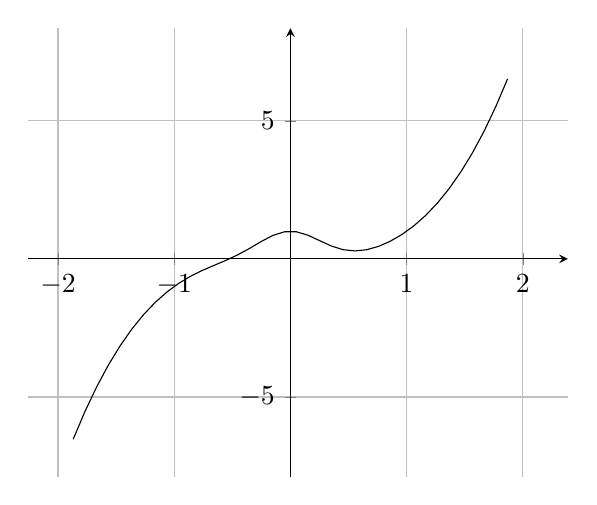
\begin{tikzpicture}
\begin{axis}[grid=both,
          xmax=2,ymax=7,
          axis lines=middle,
          restrict y to domain=-7:7,
          enlargelimits]
\addplot[domain=-5:5,samples=100]{pow(2,-10*x^2)+x^3};
\end{axis}
\end{tikzpicture}
\end{figure}
 
Take it's infinitely small fragment (in our example, an infinitely small interval for~$x$ around zero; see the rest of the book for an explanation what is infinitely small):
\begin{figure}[H]
\begin{tikzpicture}
\begin{axis}[grid=both,
          xmax=2,ymax=7,
          axis lines=middle,
          restrict y to domain=-7:7,
          enlargelimits]
\addplot[domain=-0.2:0.2,samples=100]{pow(2,-10*x^2)+x^3};
\end{axis}
\end{tikzpicture}
\end{figure}

Next consider that with a value~$y$ replaced with an infinitely small interval like $[y-\epsilon;y+\epsilon]$:
\begin{figure}[H]
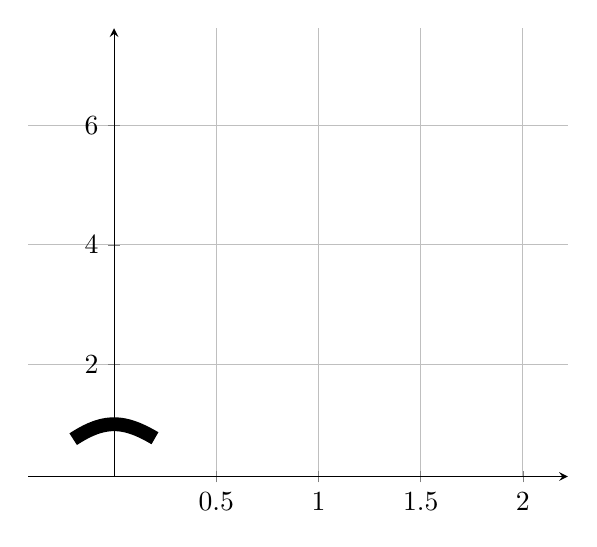
\begin{tikzpicture}
\begin{axis}[grid=both,
          xmax=2,ymax=7,
          axis lines=middle,
          restrict y to domain=-7:7,
          enlargelimits]
\addplot[domain=-0.2:0.2,samples=100,
          line width=5pt]{pow(2,-10*x^2)+x^3};
\end{axis}
\end{tikzpicture}
\end{figure}

Now we have ``an infinitely thin and short strip''. In fact, it is the same as an ``infinitely small rectangle'' (Why? So infinitely small behave, it can be counter-intuitive, but if we consider the above meditations formally, we could get this result):
\begin{figure}[H]
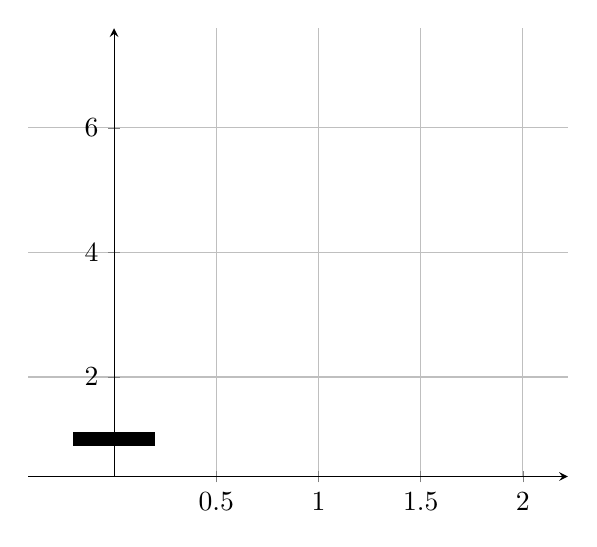
\begin{tikzpicture}
\begin{axis}[grid=both,
          xmax=2,ymax=7,
          axis lines=middle,
          restrict y to domain=-7:7,
          enlargelimits]
\addplot[domain=-0.2:0.2,samples=100,
          line width=5pt]{pow(2,-10)+1};
\end{axis}
\end{tikzpicture}
\end{figure}

This infinitely small rectangle's $y$~position uniquely characterizes the limit of our function (in our example at~$x\to 0$).

If we consider the set of all rectangles we obtain by shifting this rectangle by adding an arbitrary number to~$x$, we get
\begin{figure}[H]
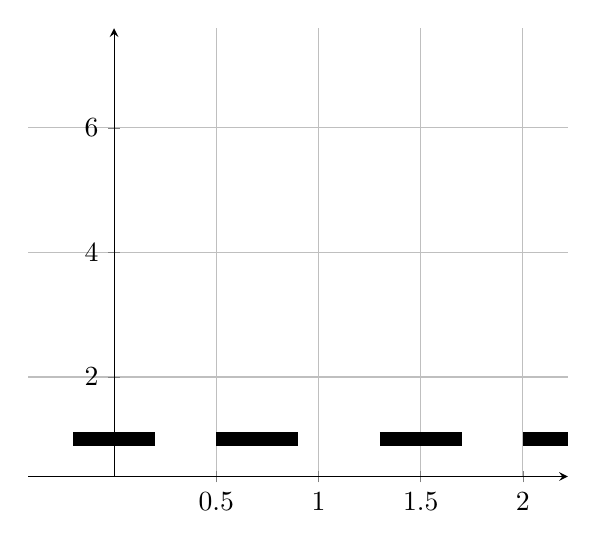
\begin{tikzpicture}
\begin{axis}[grid=both,
          xmax=2,ymax=7,
          axis lines=middle,
          restrict y to domain=-7:7,
          enlargelimits]
\addplot[domain=-0.2:0.2,samples=100,
          line width=5pt]{pow(2,-10)+1};
\addplot[domain=0.5:0.9,samples=100,
          line width=5pt]{pow(2,-10)+1};
\addplot[domain=1.3:1.7,samples=100,
          line width=5pt]{pow(2,-10)+1};
\addplot[domain=2.0:2.4,samples=100,
          line width=5pt]{pow(2,-10)+1};
\addplot[domain=2.7:3.1,samples=100,
          line width=5pt]{pow(2,-10)+1};
\addplot[domain=3.4:3.8,samples=100,
          line width=5pt]{pow(2,-10)+1};
\end{axis}
\end{tikzpicture}
\end{figure}
Such sets one-to-one corresponds to the value of the limit of our function (at $x\to 0$): Knowing such the set, we can calculate the limit (take its arbitrary element and get its so to say $y$-limit point) and knowing the limit value~($y$), we could write down the definition of this set.

So we have a formula for \emph{generalized limit}:
\[ \lim_{x\to a} f(x) =
\{ \nu \circ f|_{\Delta(a)} \circ r \mid r\in G \} \]
where~$G$ is the group of all horizontal shifts of our space~$\mathbb{R}$, $f|_{\Delta(a)}$ is the function~$f$ of which we are taking limit restricted to the infinitely small interval~$\Delta(a)$ around the point~$a$, $\nu\circ{}$~is ``stretching'' our function graph into the infinitely thin ``strip'' by applying a topological operation to it.

What all this (especially ``infinitely small'') means? It is filters and ``funcoids'' (see below for the definition).

Why we consider all shifts of our infinitely small rectangle? To make the limit not dependent of the point~$a$ to which $x$~tends. Otherwise the limit would depend on the point~$a$.

Note that for discontinuous functions elements of our set (our limit is a set) won't be infinitely small ``rectangles'' (as on the pictures), but would ``touch'' more than just one~$y$ value.

The interesting thing here is that we can apply the above formula to \emph{every} function: for example to a discontinuous function, Dirichlet function, unbounded function, unbounded and discontinuous at every point function, etc. In short, the generalized limit is defined for \emph{every} function. We have a definition of limit for every function, not only a continuous function!

And it works not only for real numbers. It would work for example for any function between two topological vector spaces (a vector space with a topology).

Hurrah! Now we can define derivative and integral of \emph{every} function.

\chapter{Funcoids}

I will reprise (without proofs) several equivalent definitions of funcoid from above in this book:

Binary relation $\delta$ between two sets (source and destination of the funcoid), conforming to the axioms:

\begin{enumerate}
\item not $\emptyset\mathrel{\delta}X$
\item not $X\mathrel{\delta}\emptyset$
\item $I\cup J \mathrel{\delta} K\iff I \mathrel{\delta}K\wedge J\mathrel{\delta}K$
\item $K\mathrel{\delta}I\cup J\iff K \mathrel{\delta}I\wedge K\mathrel{\delta}J$
\end{enumerate}

Pair of functions $(\alpha,\beta)$ between the sets of filters filters on some two sets (source and destination of the funcoid), conforming to the formula:
\[ \alpha (\mathcal{X})\sqcap \mathcal{Y}\neq \bot \iff \beta (\mathcal{Y})\sqcap \mathcal{X}\neq \bot. \]

\begin{rem}
Funcoid~$(\alpha,\beta)$ is determined by the value of~$\alpha$ (or value of~$\beta$).
\end{rem}

A function $\Delta$ from the set of subsets of some set (source of the funcoid) to the set of filters on some set (destination of the funcoid), conforming to the axioms:

\begin{enumerate}
\item $\Delta (\emptyset)=\bot$
\item $\Delta (X\sqcup Y)=\Delta (X)\sqcup \Delta (Y)$
\end{enumerate}

(Here~$\sqcup$ and~$\sqcap$ are the join and the meet correspondingly on the lattice of filters with order reverse to set-theoretic inclusion, $\bot$~is the improper filter.)

Note that we define things to have the equations:
\begin{enumerate}
\item
\begin{multline*}
X\rsuprel{f}Y \Leftrightarrow X\mathrel{\delta}Y \Leftrightarrow \\ \uparrow X\suprel{(\alpha,\beta)}\uparrow Y \Leftrightarrow
\alpha (X)\sqcap Y\neq \bot \Leftrightarrow \\ \beta (Y)\sqcap X\neq \bot
\end{multline*}
\item $\rsupfun{f}X = \Delta X = \alpha\uparrow X$
\end{enumerate}

We will denote partial orders as~$\sqsubseteq$.

I will call \emph{endofuncoid} a funcoid whose source and destination are the same.

Funcoids form a semigroup (or precategory, dependently on the exact axioms) with the operation defined by the formula:
\[ (\alpha _{1},\beta _{1})\circ (\alpha _{0},\beta _{0})=(\alpha _{1}\circ \alpha _{0},\beta _{0}\circ \beta _{1}). \]

We denote $\supfun{(\alpha,\beta)}=\alpha$ and
$(\alpha,\beta)^{-1} = (\beta,\alpha)$.

Funcoids also form a poset which is a complete lattice.

Funcoids are a generalization of both topological spaces and proximity spaces.

Also funcoids are (see above) a generalization of binary relations. (I will denote the funcoid corresponding (see above) to a binary relation~$f$ as~$\uparrow f$) This makes funcoids a common generalization for topologies/proximities and functions, so they are a convenient tool to study functions between spaces.

Another important for this article operation on funcoids is \emph{restricting} a funcoid to a filter (generalizing restricting a function to a set):~$f|_{\mathcal{X}}$ for a funcoid~$f$ and filter~$\mathcal{X}$.

Above we also have a funcoid called \emph{funcoidal product} $\mathcal{X}\times^{\mathsf{FCD}}\mathcal{Y}$ of two filters~$\mathcal{X}$ and~$\mathcal{Y}$.

\chapter{Limit for funcoids}

It is easy (see above for details) to generalize topological limit for a funcoid: a funcoid~$f$ (e.g.\ a function) \emph{tends} to point~$a$ ($f\to a$) regarding a funcoid~$\nu$ (e.g.\ to a topological or proximity space) on a filter~$\mathcal{X}$ iff
\[ \supfun{f}\mathcal{X} \sqsubseteq \supfun{\nu}\uparrow\{a\}. \]
(Here~$\uparrow$ denotes a principal filter corresponding to a set.)

More generally we can define: a funcoid~$f$ tends to a filter~$\mathcal{A}$ ($f\to\mathcal{A}$) iff $\im f\sqsubseteq\mathcal{A}$ (here $\im f = \supfun{f}\top = \supfun{f}\uparrow U$ where $U$~is the greatest set in consideration.

Then: a funcoid~$f$ tends to point~$a$ regarding a funcoid~$\nu$ on a filter~$\mathcal{X}$ iff $f|_{\mathcal{X}}$ tends to~$\uparrow\{a\}$ regarding~$\nu$.

$\lim f$ is such a point that $f$~tends to $\lim f$.

If $\nu$~is $T_2$-separable (see above), then there exists no more than one~$\lim f$.

So far, not much different than limits on topological spaces (but somehow more algebraic).

\chapter{Generalized limit}

\section{The definition of generalized limit}

Above generalized limit is defined like the formula:

\begin{equation}\label{xlim1}
\xlim f = \setcond{ \nu\circ f\circ \uparrow r}{r\in G}.
\end{equation}

We suppose:

Let $\mu$ and $\nu$ be endofuncoids (on sets~$\Ob\mu$,~$\Ob\nu$). Let $G$ be a transitive permutation
group on $\Ob\mu$.

We require that $\mu$ and every $r\in G$ commute, that is
\begin{equation}\label{commute}
\mu\circ\uparrow r=\uparrow r\circ\mu.
\end{equation}

We require for every $y\in\Ob\nu$ 
\begin{equation}\label{lim-squares}
\nu\sqsupseteq\supfun{\nu}\uparrow\{y\}\times^{\mathsf{FCD}}\supfun{\nu}\uparrow\{y\}.
\end{equation}

\begin{prop}
Formula (\ref{lim-squares}) follows from $\nu\sqsupseteq\nu\circ\nu^{-1}$.
\end{prop}

\begin{proof}
Let $\nu\sqsupseteq\nu\circ\nu^{-1}$. Then
\begin{align*}
\supfun{\nu}\uparrow\{y\}\times^{\mathsf{FCD}}\supfun{\nu}\uparrow\{y\} & =\\
\nu\circ(\uparrow\{y\}\times^{\mathsf{FCD}}\uparrow\{y\})\circ\nu^{-1} & =\\
\nu\circ\uparrow(\{y\}\times\{y\})\circ\nu^{-1} & \sqsubseteq\\
\nu\circ 1\circ\nu^{-1} & =\\
\nu\circ\nu^{-1} & \sqsubseteq\nu.
\end{align*}
(Here~$1$ is the identity element of the semigroup of endofuncoids.)
\end{proof}

\begin{rem}
The formula \eqref{lim-squares} usually works if $\nu$ is a proximity.
It does not work if $\mu$ is a topology (or more generally pretopology or preclosure). It is however easy to turn a topology into a proximity: two sets are near if they have intersecting closures.
\end{rem}

So we have (generalized) limits of arbitrary functions
acting from $\Ob\mu$ to $\Ob\nu$. (The functions in consideration
are not required to be continuous.)

\begin{rem}
Most typically $G$ is the group of translations of some topological vector space\footnote{I remind that every Banach space, every normed space, and every Hilbert space is a vector topological space.}. So in particular we have defined limit of an arbitrary function acting from a vector topological space to a topological space.
\end{rem}

\section[Injection to generalized limits]{Injection from the set of points to the set of all generalized limits}

The function $\tau$ will define an injection from the set of points
of the space $\nu$ (``numbers'', ``points'', or ``vectors'')
to the set of all (generalized) limits (i.e. values which $\xlim_{x}f$
may take).
\begin{defn}
\[ \tau(y)\eqdef\setcond{\supfun{\mu}\uparrow\{x\}\times^{\mathsf{FCD}}\supfun{\nu}\uparrow\{y\}}{x\in D}. \]
\end{defn}
\begin{prop}
\[ \tau(y)=\setcond{(\supfun{\mu}\uparrow\{x\}\times^{\mathsf{FCD}}\supfun{\nu}\uparrow\{y\})\circ\uparrow r}{r\in G} \]
for every (fixed) $x\in D$.\end{prop}

\begin{proof}
~
\begin{align*}
(\supfun{\mu}\uparrow\{x\}\times^{\mathsf{FCD}}\supfun{\nu}\uparrow\{y\})\circ\uparrow r & =\\
\supfun{\uparrow r^{-1}}\supfun{\mu}\uparrow\{x\}\times^{\mathsf{FCD}}\supfun{\nu}\uparrow\{y\} & =\\
\supfun{\mu}\supfun{\uparrow r^{-1}}\uparrow\{x\}\times^{\mathsf{FCD}}\supfun{\nu}\uparrow\{y\} & =\\
\supfun{\mu}\uparrow\{r^{-1}x\}\times^{\mathsf{FCD}}\supfun{\nu}\uparrow\{y\} & \in \\ \setcond{\supfun{\mu}\uparrow\{x\}\times^{\mathsf{FCD}}\supfun{\nu}\uparrow\{y\}}{x\in D}.
\end{align*}


Reversely
\begin{multline*}
\supfun{\mu}\uparrow\{x\}\times^{\mathsf{FCD}}\supfun{\nu}\uparrow\{y\}=\\(\supfun{\mu}\uparrow\{x\}\times^{\mathsf{FCD}}\supfun{\nu}\uparrow\{y\})\circ\uparrow e
\end{multline*}
where $e$ is the identify element of $G$.\end{proof}

\begin{prop}
\[ \tau(y)=\xlim(\supfun{\mu}\uparrow\{x\}\times^{\mathsf{FCD}}\uparrow\{y\}) \]
(for every $x$). Informally: Every $\tau(y)$ is a generalized limit
of a constant function.
\end{prop}

\begin{proof}
~
\begin{align*}
\xlim(\supfun{\mu}\uparrow\{x\}\times^{\mathsf{FCD}}\uparrow\{y\}) & =\\
\setcond{\nu\circ(\supfun{\mu}\uparrow\{x\}\times^{\mathsf{FCD}}\uparrow\{y\})\circ\uparrow r}{r\in G} & =\\
\setcond{(\supfun{\mu}\uparrow\{x\}\times^{\mathsf{FCD}}\supfun{\nu}\uparrow\{y\})\circ\uparrow r}{r\in G} & =\tau(y).
\end{align*}
\end{proof}

In further we will use on of the definitions of continuity from above:
\[ f\in\continuous(\mu,\nu)\Leftrightarrow
f\circ\mu \sqsubseteq \nu\circ f \]
and other notation from the book.

\begin{thm}
If $f$ is a function and $f|_{\supfun{\mu}\uparrow\{x\}}\in\continuous(\mu,\nu)$
and $\supfun{\mu}\uparrow\{x\}\sqsupseteq\uparrow\{x\}$
then $\xlim_{x}f=\tau(fx)$.\end{thm}

\begin{proof}
$f|_{\supfun{\mu}\uparrow\{x\}}\circ\mu\sqsubseteq\nu\circ f|_{\supfun{\mu}\uparrow\{x\}}\sqsubseteq\nu\circ f$;
thus $\langle f\rangle\supfun{\mu}\uparrow\{x\}\sqsubseteq\supfun{\nu}\supfun{f}\uparrow\{x\}$;
consequently we have
\begin{gather*}
\nu\sqsupseteq\supfun{\nu}\supfun{f}\uparrow\{x\}\times^{\mathsf{FCD}}\supfun{\nu}\supfun{f}\uparrow\{x\}\sqsupseteq\\\supfun f\supfun{\mu}\uparrow\{x\}\times^{\mathsf{FCD}}\supfun{\nu}\supfun{f}\uparrow\{x\}.\\
\begin{aligned}\nu\circ f|_{\supfun{\mu}\uparrow\{x\}} & \sqsupseteq\\
(\supfun f\supfun{\mu}\uparrow\{x\}\times^{\mathsf{FCD}}\supfun{\nu}\supfun{f}\uparrow\{x\})\circ f|_{\supfun{\mu}\uparrow\{x\}} & =\\
(f|_{\supfun{\mu}\uparrow\{x\}})^{-1}\supfun f\supfun{\mu}\uparrow\{x\}\times^{\mathsf{FCD}}\supfun{\nu}\supfun{f}\uparrow\{x\} & \sqsupseteq\\
\supfun{\id_{\dom f|_{\supfun{\mu}\uparrow\{x\}}}^{\mathsf{FCD}}}\supfun{\mu}\uparrow\{x\}\times^{\mathsf{FCD}}\supfun{\nu}\supfun{f}\uparrow\{x\} & \sqsupseteq\\
\dom f|_{\supfun{\mu}\uparrow\{x\}}\times^{\mathsf{FCD}}\supfun{\nu}\supfun{f}\uparrow\{x\} & =\\
\supfun{\mu}\uparrow\{x\}\times^{\mathsf{FCD}}\supfun{\nu}\supfun{f}\uparrow\{x\}.
\end{aligned}
\end{gather*}


$\im(\nu\circ f|_{\supfun{\mu}\uparrow\{x\}})=\supfun{\nu}\supfun{f}\uparrow\{x\}$;
\begin{align*}
\nu\circ f|_{\supfun{\mu}\uparrow\{x\}} & \sqsubseteq\\
\supfun{\mu}\uparrow\{x\}\times^{\mathsf{FCD}}\im(\nu\circ f|_{\supfun{\mu}\uparrow\{x\}}) & =\\
\supfun{\mu}\uparrow\{x\}\times^{\mathsf{FCD}}\supfun{\nu}\supfun{f}\uparrow\{x\}.
\end{align*}
So $\nu\circ f|_{\supfun{\mu}\uparrow\{x\}}=\supfun{\mu}\uparrow\{x\}\times^{\mathsf{FCD}}\supfun{\nu}\supfun{f}\uparrow\{x\}$.

Thus
\begin{multline*}
\xlim_{x}f= \\ \setcond{(\supfun{\mu}\uparrow\{x\}\times^{\mathsf{FCD}}\supfun{\nu}\supfun{f}\uparrow\{x\})\circ\uparrow r}{r\in G}= \\ \tau(fx).
\end{multline*}
\end{proof}
\begin{rem}
Without the requirement of $\supfun{\mu}\uparrow\{x\}\sqsupseteq\uparrow\{x\}$
the last theorem would not work in the case of removable singularity.\end{rem}
\begin{thm}
Let $\nu\sqsubseteq\nu\circ\nu$. If $f|_{\supfun{\mu}\uparrow\{x\}}\overset{\nu}{\rightarrow}\uparrow\{y\}$
then $\xlim_{x}f=\tau(y)$.\end{thm}

\begin{proof}
$\im f|_{\supfun{\mu}\uparrow\{x\}}\sqsubseteq\supfun{\nu}\uparrow\{y\}$;
$\supfun f\supfun{\mu}\uparrow\{x\}\sqsubseteq\supfun{\nu}\uparrow\{y\}$;
\begin{align*}
\nu\circ f|_{\supfun{\mu}\uparrow\{x\}} & \sqsupseteq\\
(\supfun{\nu}\uparrow\{y\}\times^{\mathsf{FCD}}\supfun{\nu}\uparrow\{y\})\circ f|_{\supfun{\mu}\uparrow\{x\}} & =\\
\supfun{(f|_{\supfun{\mu}\uparrow\{x\}})^{-1}}\supfun{\nu}\uparrow\{y\}\times^{\mathsf{FCD}}\supfun{\nu}\uparrow\{y\} & =\\
\supfun{\id_{\supfun{\mu}\uparrow\{x\}}^{\mathsf{FCD}}\circ f^{-1}}\supfun{\nu}\uparrow\{y\}\times^{\mathsf{FCD}}\supfun{\nu}\uparrow\{y\} & \sqsupseteq\\
\supfun{\id_{\supfun{\mu}\uparrow\{x\}}^{\mathsf{FCD}}\circ f^{-1}}\supfun f\supfun{\mu}\uparrow\{x\}\times^{\mathsf{FCD}}\supfun{\nu}\uparrow\{y\} & =\\
\supfun{\id_{\supfun{\mu}\uparrow\{x\}}^{\mathsf{FCD}}}\supfun{f^{-1}\circ f}\supfun{\mu}\uparrow\{x\}\times^{\mathsf{FCD}}\supfun{\nu}\uparrow\{y\} & \sqsupseteq\\
\supfun{\id_{\supfun{\mu}\uparrow\{x\}}^{\mathsf{FCD}}}\supfun{\id_{\supfun{\mu}\uparrow\{x\}}^{\mathsf{FCD}}}\supfun{\mu}\uparrow\{x\}\times^{\mathsf{FCD}}\supfun{\nu}\uparrow\{y\} & =\\
\supfun{\mu}\uparrow\{x\}\times^{\mathsf{FCD}}\supfun{\nu}\uparrow\{y\}.
\end{align*}

On the other hand, \[ f|_{\supfun{\mu}\uparrow\{x\}}\sqsubseteq\supfun{\mu}\uparrow\{x\}\times^{\mathsf{FCD}}\supfun{\nu}\uparrow\{y\}; \]

\begin{multline*}
\nu\circ f|_{\supfun{\mu}\uparrow\{x\}}\sqsubseteq\supfun{\mu}\uparrow\{x\}\times^{\mathsf{FCD}}\supfun{\nu}\supfun{\nu}\uparrow\{y\}\sqsubseteq\\\supfun{\mu}\uparrow\{x\}\times^{\mathsf{FCD}}\supfun{\nu}\uparrow\{y\}.
\end{multline*}

So $\nu\circ f|_{\supfun{\mu}\uparrow\{x\}}=\supfun{\mu}\uparrow\{x\}\times^{\mathsf{FCD}}\supfun{\nu}\uparrow\{y\}$.

\begin{multline*}
\xlim_{x}f=\setcond{\nu\circ f|_{\supfun{\mu}\uparrow\{x\}}\circ\uparrow r}{r\in G}=\\ \setcond{(\supfun{\mu}\uparrow\{x\}\times^{\mathsf{FCD}}\supfun{\nu}\uparrow\{y\})\circ\uparrow r}{r\in G}=\tau(y).
\end{multline*}
\end{proof}
\begin{cor}
If $\lim_{\supfun{\mu}\uparrow\{x\}}^{\nu}f=y$ then $\xlim_{x}f=\tau(y)$ (provided that $\nu\sqsubseteq\nu\circ\nu$).
\end{cor}
We have injective $\tau$ if $\supfun{\nu}\uparrow\{y_{1}\}\sqcap\supfun{\nu}\uparrow\{y_{2}\}=\bot^{\mathscr{F}(\Ob\mu)}$
for every distinct $y_{1},y_{2}\in\Ob\nu$ that is if $\nu$ is $T_{2}$-separable.

\section{Hausdorff and Kolmogorov funcoids}

\begin{defn}
A funcoid~$f$ is \emph{Kolmogorov} when
$\supfun{f}\uparrow\{x\}\ne\supfun{f}\uparrow\{y\}$ for every distinct points
$x,y\in\dom f$.
\end{defn}

\begin{defn}
\emph{Limit}~$\lim\mathcal{F}=x$ of a filter~$\mathcal{F}$
regarding funcoid~$f$ is such a point that $\supfun{f}\uparrow\{x\}\sqsupseteq\mathcal{F}$.
\end{defn}

\begin{defn}
\emph{Hausdorff} funcoid is such a funcoid that every proper
filter on its image has at most one limit.
\end{defn}

\begin{prop}
The following are pairwise equivalent for every funcoid~$f$:
\begin{enumerate}
\item\label{hd:eq-d} $f$~is Hausdorff.
\item\label{hd:eq-op}
$x\ne y\Rightarrow\supfun{f}\uparrow\{x\}\sqcap\supfun{f}\uparrow\{y\}=\bot$.
\end{enumerate}
\end{prop}

\begin{proof}
~
\begin{description}
\item[\ref{hd:eq-d}$\Rightarrow$\ref{hd:eq-op}]
If~\ref{hd:eq-op} does not hold,
then there exist distinct points~$x$ and~$y$ such that
$\supfun{f}\uparrow\{x\}\sqcap\supfun{f}\uparrow\{y\}\ne\bot$.
So~$x$ and~$y$ are both limit points of
$\supfun{f}\uparrow\{x\}\sqcap\supfun{f}\uparrow\{y\}$, and thus~$f$ is not
Hausdorff.
\item[\ref{hd:eq-op}$\Rightarrow$\ref{hd:eq-d}]
Suppose~$\mathcal{F}$ is proper.
\begin{multline*}
\supfun{f}\uparrow\{x\}\sqsupseteq\mathcal{F}\land
\supfun{f}\uparrow\{y\}\sqsupseteq\mathcal{F}\Rightarrow \\
\supfun{f}\uparrow\{x\}\sqcap\supfun{f}\uparrow\{y\}\ne\bot \Rightarrow x=y.
\end{multline*}
\end{description}
\end{proof}

\begin{cor}
Every entirely defined Hausdorff funcoid is Kolmogorov.
\end{cor}

\begin{rem}
It is enough to be ``almost entirely defined'' (having nonempty
value everywhere except of one point).
\end{rem}

\begin{obvious}
For a complete funcoid induced by a topological space this
coincides with the traditional definition of a Hausdorff
topological space.
\end{obvious}

\chapter{Operations on generalized limits}

I will call \emph{singularities} the set of generalized limits of the form $\xlim_{\supfun{\mu}\uparrow\{x\}}f$ where $f$~is an entirely defined funcoid and $x$~ranges all points of~$\Ob\mu$.

Switching back and forth between generalized limits and what I call $F$-singularities:
\begin{gather*}
\Phi f =\setcond{(\dom F, F)}{F \in \up f};\\
\Psi f = \im f.
\end{gather*}

\begin{prop}
$\Phi$ is an injection from the set of singularities to the set of monovalued functions, provided the funcoid~$\mu$ is Kolmogorov and~$\nu$ is entirely defined.
\end{prop}

\begin{proof}
That it's an injection is obvious.

We need to prove that $\dom F_0\ne\dom F_1$ for each~$F_0,F_1\in f$ such that $F_0\ne F_1$.
Really, $F_0=\nu\circ f|_{\supfun{\mu}\uparrow\{x_0\}}\circ\uparrow r_0$ for $x_0\in\Ob\mu$, $r_0\in G$.
We have $\dom F_0 = \dom f|_{\supfun{\mu}\uparrow\{x_0\}}=\supfun{\mu}\uparrow\{x_0\}$. Similarly $\dom F_1=\supfun{\mu}\uparrow\{x_1\}$ for some $x_1\in\Ob\mu$.
Thus $\dom F_0\ne\dom F_1$ because otherwise $x_0=x_1$ and so $r_0\ne r_1$,
\begin{multline*}
\dom F_0=\supfun{\uparrow r_0^{-1}}\supfun{\mu}\uparrow\{x_0\}=\\\supfun{\mu}\supfun{\uparrow r_0^{-1}}\uparrow\{x_0\}\ne\\\text{(Kolmogorov property)}\ne\\\supfun{\mu}\supfun{\uparrow r_1^{-1}}\{x_0\}=\\\supfun{\uparrow r_1^{-1}}\supfun{\mu}\{x_0\}=\dom F_1,
\end{multline*}
contradiction.
\end{proof}

So if we define a function on the set of functions whose values are funcoids, we automatically define (as this injection preimage) a function on the set of singularities. Let's do it.

Let $\varphi$ be a (possibly multivalued) multiargument function.

\section{Applying functions to functions}

As usually in calculus:

\begin{defn}
$(\varphi f) x = \varphi (\lambda i \in D : f_i x)$
for an indexed family $f$ of functions of the same domain $D$.
\end{defn}

\section{Applying functions to sets}

\begin{defn}
  $\varphi X = \rsupfun{\varphi} \prod X$ for a family $X$ of sets.
\end{defn}

\begin{obvious}
$\varphi (\lambda i \in D : \{ x_0 \}) = \{ \varphi x \}$.
\end{obvious}

\section{Applying functions to filters}

\begin{defn}
  $\varphi x = \supfun{\varphi} \prod^{\reloids}_{X \in \prod x} X$ for a
  family $x$ of atomic filters.
\end{defn}

\begin{prop}
  $\varphi$ can be continued to a pointfree funcoid.
\end{prop}

\begin{proof}
  Need to prove (theorem~\ref{pf-atom-cont})
  \[ \supfun{\varphi} \prod^{\reloids}_{X \in \prod a} X \sqsubseteq \bigsqcap
     \setcond{\bigsqcup \rsupfun{x \mapsto \supfun{\varphi}
     \prod^{\reloids}_{X \in \prod x} X} \atoms \mathcal{X}}{\mathcal{X} \in
     \up a} . \]
  Really,
\begin{multline*}
\bigsqcup \rsupfun{x \mapsto \supfun{\varphi} \prod^{\reloids}_{X \in
     \prod x} X} \atoms \mathcal{X} =\\ \supfun{\varphi} \bigsqcup \rsupfun{x
     \mapsto \prod^{\reloids}_{X \in \prod x} X} \atoms \mathcal{X} .
\end{multline*}
  But by theorem~\ref{spfn-atoms}:
  \[ \bigsqcup \rsupfun{x \mapsto \prod^{\reloids}_{X \in \prod x} X}
     \atoms \mathcal{X} = \prod^{\reloids}_{X \in \prod \mathcal{X}}
     X . \]
  So, $\bigsqcup \rsupfun{x \mapsto \prod^{\reloids}_{X \in \prod a} X}
  \atoms \mathcal{X} \sqsupseteq \prod^{\reloids}_{X \in \prod a}
  \mathcal{X}$. Thus follows the thesis.
\end{proof}

\section{Applying functions to funcoids}

\begin{defn}
For a family $f$ of funcoids and filter
  $\mathcal{X}$
\[(\varphi f) \mathcal{X} = \varphi \left( \lambda i \in \dom f :
  \supfun{f_i} \mathcal{X} \right) .\]
\end{defn}

\begin{prop}
  It is a component of a funcoid.
\end{prop}

\begin{proof}
  As composition of two components of pointfree funcoids:
  
  $\varphi (f_0, \ldots, f_n) = \varphi \circ \left( \mathcal{X} \mapsto
  \left( \lambda i \in \dom f : \supfun{f_i} \mathcal{X} \right)
  \right)$.
  
  Note that $\mathcal{X} \mapsto \left( \lambda i \in \dom f :
  \supfun{f_i} \mathcal{X} \right)$ is a component of a pointfree funcoid because
  
\begin{multline*}
  \mathcal{Y} \nasymp \left( \lambda i \in \dom f : \supfun{f_i}
  \mathcal{X} \right) \Leftrightarrow\\ \exists i \in \dom f :
  \mathcal{Y}_i \nasymp \supfun{f_i} \mathcal{X} \Leftrightarrow\\ \exists i \in
  \dom f : \mathcal{X} \nasymp \supfun{f_i^{- 1}} \mathcal{Y}_i
  \Leftrightarrow\\ \mathcal{X} \nasymp \left( \lambda i \in \dom f :
  \supfun{f_i^{- 1}} \mathcal{Y}_i \right) =\\ \mathcal{X} \nasymp \left(
  \mathcal{Y} \mapsto \left( \lambda i \in \dom f : \supfun{f_i^{- 1}}
  \mathcal{Y}_i \right) \right) \mathcal{Y}.
\end{multline*}
\end{proof}

\begin{prop}
  Applying to funcoids is consistent with applying to functions.
\end{prop}

\begin{proof}
  Consider values on principal atomic filters.
\end{proof}

\section{Applying to generalized limits}

\begin{defn}
  Define applying finitary (multivalued) functions $\varphi$ to and indexed
  family $x$ of $F$-singularities of the same domain $D$ as
  \[ \varphi x = \lambda \Delta \in D : \supfun{\nu} \varphi (\lambda i \in
     \dom x : x_i \Delta) . \]
\end{defn}

\begin{prop}
  If $\nu$ is transitive ($\nu \circ \nu \sqsubseteq \nu$) and reflexive and
  $\nu$ commutes with $\varphi$ in some argument $k$, then
  \[ \varphi x = \lambda \Delta \in D : \varphi (\lambda i \in \dom x :
     x_i \Delta) . \]
\end{prop}

\begin{proof}
  $\lambda \Delta \in D : \varphi (\lambda i \in \dom x : x_i \Delta)
  \sqsubseteq \varphi x$ because $\nu$ is reflexive.
  
  $x_i = \nu \circ f_i \circ r_i'$ for some funcoid $f_i$ and $r_i' \in G$.
  
  $x_i \Delta = \supfun{\nu} \supfun{f_i } \supfun{r_i} \Delta$ for some $r_i
  \in G$.
  
  \begin{multline*}\varphi (\lambda i \in \dom x : x_i \Delta) =\\ \varphi (\lambda i \in
  \dom x : \supfun{\nu} \supfun{f_i} \supfun{r_i} \Delta) \sqsupseteq\\
  \varphi \left( \lambda i \in \dom x : \left\{\begin{array}{ll}
    \supfun{\nu} \supfun{f_i} \supfun{r_i} \Delta & \text{if } i \neq k\\
    \supfun{\nu} \supfun{\nu} \supfun{f_i} \supfun{r_i} \Delta & \text{if } i =
    k
  \end{array}\right. \right) =\\ \supfun{\nu} \varphi \left( \lambda i \in
  \dom x : \supfun{\nu} \supfun{f_i} \supfun{r_i} \Delta \right) =
  \varphi x.\end{multline*}
\end{proof}

\begin{defn}
  Applying to singularities: $\varphi x = \Psi f (\lambda i \in \dom x :
  \Phi x_i)$ (applicable only if limits $x_i$ are taken on filters that are
  equal up to $\supfun{r}$ for $r \in G$).
\end{defn}

\begin{thm}
  If $\varphi$ is continuous regarding $\nu$ in each argument and $\dom f_0
  = \cdots = \dom f_n = \Delta$ and $\nu \circ \nu \sqsubseteq \nu$, then for singularities
\[ \lim \varphi (f_0, \ldots, f_n) = \varphi (\lim f_0, \ldots, \lim f_n). \]
\end{thm}

\begin{proof}
  We will prove instead \[ \varphi (\Phi \lim f_0, \ldots, \Phi \lim f_n) = \Phi
  \lim \varphi (f_0, \ldots, f_n). \]
  
  Equivalently transforming:
\begin{multline*}
  \lambda \Delta \in D : \supfun{\nu} \varphi ((\Phi \lim f_0) \Delta,
  \ldots, (\Phi \lim f_n) \Delta) =\\ \Phi \lim \varphi (f_0, \ldots, f_n);
\end{multline*}  

  $\nu \circ \varphi (\nu \circ f_0 \circ r, \ldots, \nu \circ f_n \circ r) =
  \nu \circ \varphi (f_0, \ldots, f_n) \circ r$;
  
  $\nu \circ \varphi (\nu \circ f_0, \ldots, \nu \circ f_n) = \nu \circ
  \varphi (f_0, \ldots, f_n)$;
  
  Obviously, $\nu \circ \varphi (\nu \circ f_0, \ldots, \nu \circ f_n)
  \sqsupseteq \nu \circ \varphi (f_0, \ldots, f_n)$.
  
  Reversely, applying continuity $n + 1$ times, we get:
\begin{multline*}
  \nu \circ \varphi (\nu \circ f_0, \ldots, \nu \circ f_n) \sqsubseteq\\
     \underset{n + 1 \text{ times}}{\underbrace{\nu \circ \nu}} \circ \varphi
     (f_0, \ldots, f_n) \sqsubseteq\\ \nu \circ \varphi (f_0, \ldots, f_n) .
\end{multline*}
  So $\nu \circ \varphi (\nu \circ f_0, \ldots, \nu \circ f_n) = \nu \circ
  \varphi (f_0, \ldots, f_n)$.
\end{proof}

\begin{prop}
If $\phi$ is continuous regarding~$\nu$ in each argument, then
\begin{multline*}
  \varphi (\lim f_0 |_{\Delta}, \ldots, \lim f_n |_{\Delta}) =\\ \lim \varphi
  (f_0 |_{\Delta}, \ldots, f_n |_{\Delta}) =\\ \lim_{\Delta} \varphi (f_0,
  \ldots, f_n)
\end{multline*}
for funcoids $f_0$, ..., $f_n$,

\end{prop}

\begin{proof}
  The first equality follows from the above.
  
  It remains to prove \[ \varphi (f_0 |_{\Delta}, \ldots, f_n |_{\Delta}) =
  (\varphi (f_0, \ldots, f_n)) |_{\Delta}. \]
  
  Equivalently transforming,
  
  $\supfun{\varphi (f_0 |_{\Delta}, \ldots, f_n |_{\Delta})} \mathcal{X} =
  \supfun{(\varphi (f_0, \ldots, f_n)) |_{\Delta}} \mathcal{X}$;
  
\begin{multline*}
  \varphi \left( \supfun{f_0 |_{\Delta}} \mathcal{X}, \ldots, \supfun{f_n
  |_{\Delta}} \mathcal{X} \right) =\\ \supfun{\varphi (f_0, \ldots, f_n)}
  (\Delta \sqcap \mathcal{X});
\end{multline*}
  
\begin{multline*}
  \varphi \left( \supfun{f_0} (\Delta \sqcap \mathcal{X}), \ldots,
  \supfun{f_n} (\Delta \sqcap \mathcal{X}) \right) =\\ \varphi \left(
  \supfun{f_0} (\Delta \sqcap \mathcal{X}), \ldots, \supfun{f_n} (\Delta
  \sqcap \mathcal{X}) \right) (\Delta \sqcap \mathcal{X}).
\end{multline*}
\end{proof}

\begin{thm}
Let~$\Delta$ be a filter on~$\mu$.
Let~$S$ be the set of all functions $p\in\mathsf{FCD}(\Ob\mu,\Ob\nu)$
such that $\dom p=\Delta$.
Let $f$, $g$ be
finitary multiargument functions on $\Ob\nu$.
Let $J$ be an index
set. Let $k \in J^{\operatorname{dom} P}$, $l \in J^{\operatorname{dom} Q}$. Then
\begin{multline*}
\forall x \in (\Ob\nu)^J : f (\lambda i \in \operatorname{dom} f : x_{k_i}) =\\ g (\lambda
   i \in \operatorname{dom} g : x_{l_i})
\end{multline*}
implies
\begin{multline*}
   \forall x \in (\rsupfun{\lim}S)^J : f (\lambda i \in
   \operatorname{dom} f : x_{k_i}) =\\ g (\lambda i \in \operatorname{dom} g : x_{l_i}) ,
\end{multline*}
provided that~$f$ and~$g$ are continuous regarding~$\nu$ in each argument.
\end{thm}

\begin{rem}
This theorem implies that if $\Ob\nu$ is a group, ring, vector space, etc., then $\rsupfun{\lim}S$ is also accordingly a group, ring, vector space, etc.
\end{rem}

\begin{proof}
Every $x_{j_i} = \lim_{\Delta} t$ for some function~$t$.

By proved above, \[ f (\lambda i \in \operatorname{dom} f : x_{k_i}) = \lim_{\Delta} f(\lambda i \in \operatorname{dom} f : t_{k_i}). \]

It's enough to prove \[ f(\lambda i \in \operatorname{dom} f : t_{k_i}) = g(\lambda i \in \operatorname{dom} f : t_{l_i}). \]
But that's trivial.
\end{proof}

\begin{conjecture}
The above theorem stays true if $S$~is instead a set of limits of monovalued funcoids.
\end{conjecture}

\section{Applications}

Having generalized limit, we can in an obvious way define derivative of an arbitrary function.

We can also define definite integral of an arbitrary function (I remind that integral is just a limit on a certain filter). The result may differ dependently on whether we use Riemann and Lebesgue integrals.

From above it follows that my generalized derivatives and integrals are linear operators.

\chapter{Hierarchy of singularities}

Above we have defined (having fixed endofuncoids~$\mu$ and~$\nu$) for every set of ``points''~$R=\Ob\nu$ its set of singularities $\operatorname{SNG}(R)$.

We can further consider
\[
\operatorname{SNG}(\operatorname{SNG}(R)), \operatorname{SNG}(\operatorname{SNG}(\operatorname{SNG}(R))),
\]
etc.

If we try to put our generalized derivative into say the differential equation $h\circ f'=g\circ f$ on real numbers, we have a trouble: The left part belongs to the set of functions to $\operatorname{SNG}(Y)$ and the right part to the set of functions to~$Y$, where $Y$ is the set of solutions. How to equate them? If $Y$~would be just~$\mathbb{R}$ we would take the left part of the type $\operatorname{SNG}(\mathbb{R})$ and equate them using the injection~$\tau$ defined above. But stop, it does not work: if the left part is of $\operatorname{SNG}(\mathbb{R})$ then the right part, too. So the left part would be $\operatorname{SNG}(\operatorname{SNG}(\mathbb{R}))$, etc.\ infinitely.

So we need to consider the entire set (\emph{supersingularities})
\[
\operatorname{SUPER}(R) =
R\cup\operatorname{SNG}(R)\cup
\operatorname{SNG}(\operatorname{SNG}(R))\cup\dots
\]

But what is the limit (and derivative) on this set? And how to perform addition, subtraction, multiplication, division, etc.\ on this set?

Finite functions on the set $\operatorname{SUPER}(R)$ are easy: just apply~$\tau$ to arguments belonging to ``lower'' parts of the hierarchy of singularities a finite number of times, to make them to belong to the same singularity level (the biggest singularity level of all arguments).

Instead of generalized limit, we will use ``regular'' limit but on the set $\operatorname{SUPER}(R)$ (which below we will make into a funcoid) rather than on the set~$R$.

See? We have a definition of (finite) differential equations (even partial differential equations) for discontinuous functions. It is just a differential equation on the ring~$\operatorname{SUPER}(R)$ (if~$R$ is a ring).

What nondifferentiable solutions of such equations do look like? No idea! Do they contain singularities of higher levels of the above hierarchy? What about singularities in our sense at the center of a blackhole (that contain ``lost'' information)? We have something intriguing to research.

\chapter{Funcoid of singularities}

I remind that for funcoid~$\nu$ the relation~$\rsuprel{\nu}$ can be thought as generalized nearness.

We will extend $\rsuprel{\nu}$ from the set~$R$ of points to the set of funcoids from a (fixed) set~$A$ to~$R$ having the same domain (or empty domain):
\[
y_0 \rsuprel{\nu} y_1 \Leftrightarrow
\forall x\in\atoms\dom y_0:
\supfun{y_0}x \rsuprel{\nu} \supfun{y_1}x
\]
where $\atoms\dom y_0$ is the set of ultrafilters over the filter $\dom y_0$.

The above makes $\nu$ a pointfree funcoid on this set of funcoids:

\begin{proof}
Because funcoids are isomorphic to filters on certain boolean lattice, it's enough to prove:
\begin{align*}
\lnot(\bot\rsuprel{\nu}y_1),\quad
\lnot(y_0\rsuprel{\nu}\bot),\\
i\sqcup j\rsuprel{\nu}y_1 \Leftrightarrow
i\rsuprel{\nu}y_1\lor j\rsuprel{\nu}y_1,\\
y_0\rsuprel{\nu}i\sqcup j \Leftrightarrow
y_0\rsuprel{\nu}i\lor y_0\rsuprel{\nu}j.
\end{align*}
The first two formulas are obvious. Let's prove the third (the fourth is similar):
\begin{multline*}
i\sqcup j\rsuprel{\nu}y_1 \Leftrightarrow\\
\forall x\in\atoms\dom(i\sqcup j):
\supfun{y_0}x \rsuprel{\nu} \supfun{y_1}x \Leftrightarrow\\
\forall x\in\atoms(\dom i\sqcup\dom j):
\supfun{y_0}x \rsuprel{\nu} \supfun{y_1}x \Leftrightarrow\\
\forall x\in\atoms\dom i\cup\atoms\dom j:\\
\supfun{y_0}x \rsuprel{\nu} \supfun{y_1}x \Leftrightarrow\\
\forall x\in\atoms\dom i:
\supfun{y_0}x \rsuprel{\nu} \supfun{y_1}x \lor\\
\forall x\in\atoms\dom j:
\supfun{y_0}x \rsuprel{\nu} \supfun{y_1}x \Leftrightarrow\\
i\rsuprel{\nu}y_1\lor j\rsuprel{\nu}y_1.
\end{multline*}
\end{proof}

We will define two singularities being ``near'' 
in terms of $F$-singularities (that are essentially the same as singularities):

Two $F$-singularities~$y_0$,~$y_1$ are near iff
there exist two elements of~$y_0$ and~$y_1$ correspondingly such that $\dom y_0=\dom y_1$ and every $Y_0\in y_0$, $Y_1\in y_1$ are near.

Let's prove it defines a funcoid on the set of $F$-singularities:

\begin{proof}
Not $\emptyset\rsuprel{\nu}X$ and not $X\rsuprel{\nu}\emptyset$ are obvious.

It remains to prove for example
\[ I\cup J\rsuprel{\nu}K \Leftrightarrow 
I\rsuprel{\nu}K \lor J\rsuprel{\nu}K, \]
but that's obvious.
\end{proof}

\chapter{Funcoid of supersingularities}

It remains to define the funcoid of supersingularities.

Let $y_0$,~$y_1$ be sets of supersingularities.

We will define $y_0$~and~$y_1$ to be near iff
there exist natural~$n$,~$m$ such that
\[ \tau^n[y_0\cap\operatorname{SNG}^m(R)] \rsuprel{\nu}
\tau^m[y_1\cap\operatorname{SNG}^n(R)]. \]

\begin{rem}
In this formula both the left and the right arguments of~$\rsuprel{\nu}$ belong to $\operatorname{SNG}^{n+m}(R)$.
\end{rem}

Let's prove that the above formula really defines a funcoid:

\begin{proof}
We need to show
\begin{align*}
\emptyset\rsuprel{\nu}y_1,\quad
y_0\rsuprel{\nu}\emptyset,\\
i\cup j\rsuprel{\nu}y_1 \Leftrightarrow
i\rsuprel{\nu}y_1\lor j\rsuprel{\nu}y_1,\\
y_0\rsuprel{\nu}i\cup j \Leftrightarrow
y_0\rsuprel{\nu}i\lor y_0\rsuprel{\nu}j.
\end{align*}
The first two formulas are obvious. Let's prove the third (the fourth is similar):
\begin{align*}
&i\cup j\rsuprel{\nu}y_1 \Leftrightarrow \\&
\exists n,m\in\mathbb{N}:\\& 
\tau^n[(i\cup j)\cap\operatorname{SNG}^m(R)] \rsuprel{\nu}
\tau^m[y_1\cap\operatorname{SNG}^n(R)] \Leftrightarrow \\&
\exists n,m\in\mathbb{N}:\\& 
\tau^n[(i\cap\operatorname{SNG}^m(R))\cup(j\cap\operatorname{SNG}^m(R)))] \rsuprel{\nu}\\&
\tau^m[y_1\cap\operatorname{SNG}^n(R)] \Leftrightarrow \\&
\exists n,m\in\mathbb{N}:\\& 
\tau^n[i\cap\operatorname{SNG}^m(R)]\cup\tau^n[j\cap\operatorname{SNG}^m(R)))] \rsuprel{\nu}\\&
\tau^m[y_1\cap\operatorname{SNG}^n(R)] \Leftrightarrow \\&
\exists n,m\in\mathbb{N}:\\& 
(\tau^n[i\cap\operatorname{SNG}^m(R)]\rsuprel{\nu}
\tau^m[y_1\cap\operatorname{SNG}^n(R)] \lor \\&
\tau^n[j\cap\operatorname{SNG}^m(R)]\rsuprel{\nu}
\tau^m[y_1\cap\operatorname{SNG}^n(R)]) \Leftrightarrow \\&
\exists n,m\in\mathbb{N}:\\& 
\tau^n[i\cap\operatorname{SNG}^m(R)]\rsuprel{\nu}
\tau^m[y_1\cap\operatorname{SNG}^n(R)] \lor \\&
\exists n,m\in\mathbb{N}:\\& 
\tau^n[j\cap\operatorname{SNG}^m(R)]\rsuprel{\nu}
\tau^m[y_1\cap\operatorname{SNG}^n(R)] \Leftrightarrow \\&
i\rsuprel{\nu}y_1\lor j\rsuprel{\nu}y_1.
\end{align*}
\end{proof}

\chapter{Example differential equation}

\begin{defn}
I will call a function $f$ \emph{pseudocontinuous} on $D$ when \[ \forall a \in D :
\xlim_{\Delta \{ a \} \setminus \{ a \}} f = f (a). \]
\end{defn}

\section{Arbitrary pseudocontinuous continuations}

Note that arbitrary pseudocontinuous continuations of generalized solutions of differential equations (diffeqs) are silly:

Let $A(f(x), f'(x))=0$ is a diffeq and let the equality is undefined at some point (e.g.\ contains division by zero). Let $f$ be its solution with derivative~$f'$.
Replace the value in undefined point~$x$ of the solution by an arbitrary value~$y$ and calculate the derivative $y'$ at this point. No need to hold $A(y,y')=0$ at this point because the point is outside of the domain of the original solution. Then replace in our solution~$f$ the value at this point~$x$ by~$y$ and the derivative by $y'$. Then we have another continuation of the solution because the equality $A(f(x), f'(x))=0$ holds both for the point~$x$ and all other points.

Thus, we can take any solution and add one point of it with an arbitrary value. That's largely a nonsense from the practical point of view. (Why we would arbitrarily change one point of the solution?)

\section{Solutions with pseudocontinuous derivative}

So I will require for generalized solutions instead that the derivative~$f'$ is pseudocontinuous.

Next, we will consider a particular example, the diffeq $y'(x)=-1/x^2$. Let us find its continuations of generalized solutions~$y$ to the entire real line (including $x=0$) with a $y'$ being pseudocontinuous.

As it's well known, its solutions in the traditional sense are
$y (x) = c_1 + \frac{1}{x}$ for $x < 0$ and $y (x) = c_2 + \frac{1}{x}$ for $x
> 0$ where $c_1$,~$c_2$ are arbitrary constants. The derivative is $y'(x)=-1/x^2$.

\begin{rem}
We could consider solutions on the space of supersingularities and it would be the same, except that we would be allowed to take~$c_1$,~$c_2$ arbitrary supersingularities instead of real numbers. This is because the supersingularities form a ring and thus the algorithm of solving the diffeq is the same as for the real numbers, thus producing the solutions of the same form.
\end{rem}

Let's find the pseudocontinuous generalized derivative at zero by pseudocontinuity:
\[ y'(0) = \lim_{x\to 0} \frac{1}{x^2}. \]

On the other hand, by the definition of derivative
\[ y'(0) = \lim_{\varepsilon \rightarrow 0}  \frac{c_i + \frac{1}{\varepsilon} - f
(0)}{\varepsilon}. \]

The equality is possible only when $c_1=c_2=c=f(0)$.

So, finally, our solution is $y(x) = c + \frac{1}{x}$ for $x\ne 0$ and $y(0)=c$.

A thing to notice that now the solution is ``whole'': it exists at zero and does not split to two ``branches'' with independent constants. Our $y(x)$ is a real function, but the derivative has a singularity in my sense.

We considered generalized solutions with pseudocontinuous derivative. It is apparently the right way to define a class of generalized solutions. Now I will consider also several apparently wrong classes of solutions.

\section{Pseudocontinuous generalized solutions}

Let us try to require the solution of our diffeq to be pseudocontinuous instead of its derivative to be pseudocontinuous.

We already have the solution for nonzero points. For zero:
\[ y'(0) = \lim_{x\to 0}(-1/x^2). \]

So the derivative:
\begin{multline*}
y' (0) = \lim_{x\to 0} \frac{y(x) - y(0)}{x} =\\ \lim_{x\to 0} \frac{y(x)}{x} - \lim_{x\to 0} \frac{y(0)}{x} =\\ \lim_{x\to 0} \frac{1}{x^2} - \lim_{x\to 0} \frac{y(0)}{x}.
\end{multline*}

The equality is impossible.

\part{Postface}
\include{chap-postface}
\include{chap-prize}
\include{chap-story}

\include{appendixes}

\printindex{}

\bibliographystyle{plain}
\bibliography{refs}

% TODO: move to the preamble
\addtocounter{figure}{-1}
\refstepcounter{figure}\label{LASTFIGURE}

\end{document}
